% \documentclass[handout]{beamer}
\documentclass{beamer}
\usetheme{CambridgeUS}
\usefonttheme{serif}
\setbeamertemplate{navigation symbols}{}

\usepackage{ctex}
\usepackage{amsmath,amssymb,amsfonts,bm}
\usepackage{graphicx,subfigure}
\usepackage{adjustbox}
\usepackage{color,xcolor}
\usepackage{tikz}
\usepackage{animate}

\newcommand{\ANIMATE}{}
\ifdefined \ANIMATE
\newcommand{\dongtu}[1]{#1}
\else
\newcommand{\dongtu}[1]{}
\fi


% 自定义数学公式
\newcommand{\abs}[1]{\left\vert#1\right\vert}
\newcommand{\floor}[1]{\left\lfloor{#1}\right\rfloor}
\newcommand{\ceil}[1]{\left\lceil{#1}\right\rceil}
\newcommand{\sbrace}[1]{\left(#1\right)}
\newcommand{\mbrace}[1]{\left[#1\right]}
\newcommand{\bbrace}[1]{\left\{#1\right\}}
\newcommand{\eval}[2]{\left.{#1}\right|_{#2}}
\newcommand{\conj}[1]{{\rm conj}\sbrace{#1}}
\newcommand{\ALLP}{\mathcal{A}}
\newcommand{\PS}{\mathcal{P}}
\newcommand{\dd}[1]{\mathrm{d}#1}
\newcommand{\ii}[1]{\int\!{#1\dd x}}
\newcommand{\VecNorm}[1]{\left\Vert#1\right\Vert}% 向量模
\newcommand{\spell}[1]{#1}
\newcommand{\up}[1]{^{(#1)}}
\newcommand{\TT}{^\top}% 矩阵转置
\newcommand{\OO}{\ensuremath{\mathbb O}}% n 阶展开多项式余项
\newcommand{\OC}{\ensuremath{\mathcal O}}% 算法复杂度
\newcommand{\lfrac}[2]{#1/#2}
\newcommand{\DIF}[1]{\ensuremath{\frac{\partial}{\partial #1}}}
\newcommand{\DIFF}[2]{\ensuremath{\frac{\partial #1}{\partial #2}}}
\newcommand{\cd}[1]{\,\texttt{#1}\,}
\newcommand{\dbrace}[1]{
  \Bigl\{
    #1
  \Bigr\} 
}
\newcommand{\Painleve}{Painlev{\'e}}
\newcommand{\red}[1]{{\color{red}#1}}
\usepackage{textcomp}
\newcommand{\tpa}{\checkmark}
\newcommand{\tpb}{$-$}
\newcommand{\tpc}{\texttimes}

\title[华东师范大学硕士学位论文]{构造非线性系统精确解的相关机械化算法研究}
\author[余江涛]{余江涛 \and \\导师: 柳银萍~教授}
\date{\today}

\begin{document}
\frame{
    \tikz[overlay,remember picture]\node[opacity=0.1]at (current page.center){
\includegraphics[width=0.7\paperheight]{../paper/sty/ecnu_logo.pdf}};
    \titlepage
}

\section{本文工作}
\begin{frame}
\frametitle{本文工作}
\begin{figure}
\centering
\includegraphics[height=0.8\textheight]{fig/ppt-outline.pdf} 
\end{figure}
\end{frame}

\section{构造非线性演化方程三种波解}
\begin{frame}{构造非线性演化方程三种波解}
\begin{columns}
\begin{column}{0.5\textwidth}
  \begin{figure}
    \centering
    \includegraphics[height=0.7\textheight]{fig/outline-p1.pdf}
  \end{figure}
\end{column}
\begin{column}{0.5\textwidth}
  \begin{enumerate}
  \item 非线性演化方程
  \item \Painleve{}展开
  \item 孤子解
  \item 呼吸子解 
  \item Lump 解
  \end{enumerate}
\end{column}
\end{columns}
\end{frame}

\subsection{非线性演化方程}
\begin{frame}{非线性演化方程}
考虑(2+1)维 BKP方程
\begin{equation}
\begin{aligned}
0&=u_t+u_{xxxxx}-5u_{xxy}-5\int{u_{yy}\dd{x}}+15u_xu_{xx}\\
&+15uu_{xxx}-15uu_y-15u_x\int{u_y\dd{x}}+45u^2u_x, \label{BKP}
\end{aligned}
\end{equation}
\pause 
\begin{equation}
  u=v_x
\end{equation}
\pause 
\begin{equation}
\begin{aligned}
0&=v_{tx}+v_{xxxxxx}-5v_{xxxy}-5v_{yy}+15v_{xx}v_{xxx}\\
&+15v_xv_{xxxx}-15v_xv_{xy}-15v_{xx}v_y+45v_x^2v_{xx}. 
\end{aligned}
\end{equation}
\end{frame}

\subsection{\Painleve{}展开}
\begin{frame}{\Painleve{}展开}
\small  
\pause 
\begin{equation}
  v=\sum_{k=1}^m{\frac{u_k}{f^{m-k+1}}}=\frac{u_1}{f^m}+\cdots+\frac{u_m}{f}
\end{equation}
\pause 
\[
\begin{aligned}
0&=v_{tx}+\red{v_{xxxxxx}}-5v_{xxxy}-5v_{yy}+15v_{xx}v_{xxx}\\
&+15v_xv_{xxxx}-15v_xv_{xy}-15v_{xx}v_y+\red{45v_x^2v_{xx}}.
\end{aligned}
\]
\pause 
\[
  [m+2,\red{m+6},m+4,m+2,2m+5,2m+5,2m+3,2m+3,\red{3m+4}]
\]
\pause 
\begin{equation}
  m+6=3m+4 \Rightarrow m=1 \Rightarrow v=\frac{2f_x}{f}=2\sbrace{\ln(f)}_x 
\end{equation}
\pause 
\begin{equation}
\begin{aligned}
0&=2\,{{f}_{txx}}\,{f}^{2}+2\,{{f}_{xxxxxxx}}\,{f}^{2}-10\,{{f}_{xxxxy}}\,{f}^{2}-10\,{{f}_{xyy}}\,{f}^{2}-2\,{{f}_{xx}}\,{{f}_{t}}\,f\\
&-4\,{{f}_{tx}}\,{{f}_{x}}\,f-14\,{{f}_{xxxxxx}}\,{{f}_{x}}\,f+40\,{{f}_{xxxy}}\,{{f}_{x}}\,f+10\,{{f}_{x}}\,{{f}_{yy}}\,f+18\,{{f}_{xxxxx}}\,{{f}_{xx}}\,f\\
&-10\,{{f}_{xxxx}}\,{{f}_{xxx}}\,f-20\,{{f}_{xxx}}\,{{f}_{xy}}\,f+10\,{{f}_{xxxx}}\,{{f}_{y}}\,f+20\,{{f}_{xy}}\,{{f}_{y}}\,f+4\,{{{f}_{x}}}^{2}\,{{f}_{t}}\\
&+24\,{{f}_{xxxxx}}\,{{{f}_{x}}}^{2}-60\,{{f}_{xxy}}\,{{{f}_{x}}}^{2}-60\,{{f}_{xxxx}}\,{{f}_{x}}\,{{f}_{xx}}+60\,{{f}_{xx}}\,{{f}_{x}}\,{{f}_{xy}}+40\,{{{f}_{xxx}}}^{2}\,{{f}_{x}}\\
&-20\,{{f}_{xxx}}\,{{f}_{x}}\,{{f}_{y}}-20\,{{f}_{x}}\,{{{f}_{y}}}^{2}
\end{aligned}
\end{equation}
\end{frame}

\subsection{孤子解}
\dongtu{
\begin{frame}{孤子解}
\begin{figure}
\centering
\subfigure[扭状孤子]{
    \animategraphics[loop,autoplay,width=0.45\textwidth,poster=11]{8}{fig/(2+1)BKP-T-001/}{001}{024}
}    
\subfigure[钟状孤子]{
    \animategraphics[loop,autoplay,width=0.45\textwidth,poster=11]{8}{fig/(2+1)BKP-001/}{001}{024}
}    
\end{figure}
\end{frame}
}


\subsection{Hirota方法}
\begin{frame}{Hirota方法}
\pause
\begin{equation}
  \xi_i=k_i\sbrace{x+p_i y + q_i z + \cdots + \omega t}+c_i
\end{equation}
\pause
\begin{equation}
\begin{aligned}
f_1&=1+\exp\sbrace{\xi_1} \\ 
f_2&=1+\exp\sbrace{\xi_1}+\exp\sbrace{\xi_2}+h_{1,2}\exp\sbrace{\xi_1+\xi_2} \\ 
f_3&=1+\exp(\xi_1)+\exp(\xi_2)+\exp(\xi_3)\\
  &+h_{1,2}\exp(\xi_1+\xi_2)+h_{2,3}\exp(\xi_2+\xi_3)+h_{1,3}\exp(\xi_1+\xi_3)\\
  &+h_{1,2}h_{2,3}h_{1,3}\exp(\xi_1+\xi_2+\xi_3)
\end{aligned}
\end{equation}
\pause
\begin{equation}
\begin{aligned}
  f_{n}&=\sum_{\mu=0,1}\exp\sbrace{\sum_{i=1}^n{\mu_i \xi_i}+\sum_{1\le i<j\le n}{\mu_i\mu_jH_{i,j}}} \\ 
  &=\sum_{P\subseteq \bbrace{1,\cdots,n}}\mbrace{\sbrace{\prod_{\bbrace{i,j}\subseteq P}{h_{i,j}}}\exp\sbrace{\sum_{k\in P}{\xi_k}}} \\ 
\end{aligned}
\end{equation}
\end{frame}

\dongtu{
\begin{frame}
\begin{figure}
\animategraphics[loop,autoplay,width=0.6\textwidth,poster=13]{8}{fig/(2+1)BKP-003/}{001}{024}
\caption{3-孤子解}
\end{figure}
\end{frame}
}

\begin{frame}{改进的$n$孤子解公式}
\begin{equation}
  \xi=p_1(x_1+p_2x_2+\cdots+p_d x_d+\omega t)+p_{d+1}
\end{equation}
\begin{equation}
\PS\subseteq \ALLP=\bbrace{1,2,\cdots,d,d+1} ,
\end{equation}
\begin{equation}
S\sbrace{e,i;\PS}=\left\{\begin{array}{ll}
  p_k \to p_{k,i}, & k \in \PS ,\\ 
  p_k \to p_k , & k \not\in\PS .
\end{array}\right.
\end{equation}
\begin{equation}
  \xi_i=S(\xi,i;\PS)
\end{equation}
\end{frame}

\begin{frame}
\frametitle{改进的理由}
\begin{columns}
\begin{column}{0.65\textwidth}
\begin{table}
\centering
\small 
\begin{tabular}{lcccc}
\hline
\multicolumn{1}{c}{方程名} & 1 & 12 & 13 & 123 \\ 
\hline
(1+1)KdV & \tpa\tpb & & & \\
(2+1)BKP-T & \tpa\tpb & \tpa\tpa & & \\
(2+1)KP &\tpa\tpb &\tpa\tpa & & \\
(2+1)SK &\tpa\tpb &\tpa\tpa & & \\
(4+1)Fokas-T-2 &\tpa\tpb &\tpa\tpa & & \\
(2+1)CBS & \tpa\tpb & \tpa\tpb & & \\
(2+1)CBS-G & \tpa\tpb & \tpc\tpc & & \\
(3+1)BKP &\tpa\tpb &\tpa\tpa &\tpa\tpa &\tpc\tpc \\
(3+1)KP &\tpa\tpb &\tpa\tpa &\tpa\tpa &\tpc\tpc \\
(3+1)JM &\tpa\tpb &\tpa\tpa &\tpa\tpb &\tpc\tpc \\
(3+1)NEE-T &\tpa\tpb &\tpa\tpa &\tpa\tpb &\tpc\tpc \\
(3+1)YTSF &\tpa\tpb &\tpa\tpa &\tpa\tpb &\tpb\,\tpb \\
(3+1)CBS &\tpa\tpb &\tpa\tpb &\tpa\tpb &\tpa\tpb \\
(4+1)Fokas-T &\tpa\tpb &\tpa\tpb &\tpa\tpb &\tpc\tpc \\
\hline
\end{tabular}
\end{table}
\end{column}
\begin{column}{0.35\textwidth}
\begin{itemize}
\item `\tpa{}' 表示能够满足原方程.
\item `\tpb{}' 表示有解不能得到解.
\item `\tpc{}' 表示有解但不满足原方程.
\item 第一个对应3孤子解, 第二个对应2 lump解.
\end{itemize}
\end{column}
\end{columns}
\end{frame}

\subsection{呼吸子解}
\begin{frame}{呼吸子解}
\begin{equation}
\begin{aligned}
f_2&=1+\exp\sbrace{\xi_1}+\exp\sbrace{\xi_2}+h\exp\sbrace{\xi_1+\xi_2} \\ 
&=1+\exp(a+bI)+\exp(a-bI)+h\exp(a+bI+a-bI) \\ 
&=1+2\exp(a)\cos(b)+h\exp(2a).
\end{aligned}
\end{equation}
\end{frame}

\dongtu{
\begin{frame}
\begin{figure}
\setcounter{subfigure}{0}
\subfigure[扭状孤子对应的呼吸子解]{
  \animategraphics[loop,autoplay,width=0.45\textwidth,poster=11]{8}{fig/(2+1)BKP-T-010/}{001}{024}
}
\subfigure[钟状孤子对应的呼吸子解]{
  \animategraphics[loop,autoplay,width=0.45\textwidth,poster=11]{8}{fig/(2+1)BKP-010/}{001}{024}
}
\end{figure}
\end{frame}

\begin{frame}
\begin{figure}
\animategraphics[loop,autoplay,width=0.6\textwidth,poster=11]{8}{fig/(2+1)BKP-020/}{001}{024}
\caption{2-呼吸子解}
\end{figure}
\end{frame}
}

\subsection{Lump 解}
\dongtu{
\begin{frame}{呼吸子解取极限}
\begin{figure}
\setcounter{subfigure}{0}
\subfigure[呼吸子取极限]{
  \animategraphics[loop,autoplay,width=0.45\textwidth,poster=11]{8}{fig/(2+1)BKP-delta-010/}{001}{024}
}
\subfigure[lump 解]{
  \includegraphics[width=0.45\textwidth]{fig/(2+1)BKP-delta-010/lump.png}
}
\end{figure}
\end{frame}

\begin{frame}{lump解}
\begin{figure}
\setcounter{subfigure}{0}
\subfigure[扭状孤子对应的lump解]{
  \animategraphics[loop,autoplay,width=0.45\textwidth,poster=11]{8}{fig/(2+1)BKP-T-100/}{001}{024}
}
\subfigure[钟状孤子对应的lump解]{
  \animategraphics[loop,autoplay,width=0.45\textwidth,poster=11]{8}{fig/(2+1)BKP-100/}{001}{024}
}
\end{figure}
\end{frame}
}

\begin{frame}{lump解公式}
\begin{equation}
\begin{aligned}
\theta_i &= \eval{\frac{\partial \xi_i}{\partial p_{1,i}}}{p_{1,i}=0}, \\
b_{i,j}&= \eval{\frac{\partial^2}{\partial p_{1,i}\partial p_{1,j}}h_{i,j}}{p_{1,i}=0,p_{1,j}=0}.
\end{aligned}
\end{equation}
\begin{equation}
\begin{aligned}
\Theta_1&=\theta_{1}\theta_{2}+b_{12} \\
\Theta_2&=\theta_{1}\theta_{2}\theta_{3}\theta_{4}+b_{12}\theta_{3}\theta_{4}+b_{13}\theta_{2}\theta_{4}+b_{14}\theta_{2}\theta_{3}+b_{23}\theta_{1}\theta_{4}\\
&+b_{24}\theta_{1}\theta_{3}+b_{34}\theta_{1}\theta_{2}+b_{12}b_{34}+b_{13}b_{34}+b_{14}b_{23}
\end{aligned}
\end{equation}
\end{frame}

\begin{frame}{改进 lump 解公式}
\begin{equation}
\begin{aligned}
\Theta_m&=\prod_{k=1}^{2m}\theta_k+\frac{1}{2}\sum_{i,j}{b_{i,j}}\prod_{J\neq i,j}{\theta_J}+\frac{1}{2! 2^2}\sum_{i,j,k,l}{b_{i,j}b_{k,l}}\prod_{J\neq i,j,k,l}{\theta_{J}}+\cdots \\
&+\frac{1}{s!2^s}\sum_{i,j,\cdots,u,v}\underbrace{{b_{i,j}b_{k,l}\cdots b_{u,v}}}_{s}\prod_{J\neq i,j,\cdots, u,v}{\theta_J}+\cdots 
\end{aligned}
\end{equation}
\pause 
\vfill
\begin{equation}
f_{m-lump}=\sum_{l=0}^m\sum_{s\in L(l)}\sbrace{\prod_{k=1}^l{b_{s_{2k-1},s_{2k}}}\prod_{p\not\in s}{\theta_p}}
\end{equation}
\begin{equation*}
  L(l)=\bbrace{\sbrace{s_1, s_2, \cdots ,s_{2l}}\left|s_{2k}>s_{2k-1},s_{2k+1}>s_{2k-1},s_k\in \bbrace{1,\cdots,2l}\right.}
\end{equation*}
\end{frame}

\begin{frame}
\small
\[
\renewcommand{\arraystretch}{0.8} 
\begin{array}{l}
\Theta_3=\theta_{{1}}\theta_{{2}}\theta_{{3}}\theta_{{4}}\theta_{{5}}\theta_{{6}}
+b_{{12}}\theta_{{3}}\theta_{{4}}\theta_{{5}}\theta_{{6}}
+b_{{13}}\theta_{{2}}\theta_{{4}}\theta_{{5}}\theta_{{6}}
+b_{{14}}\theta_{{2}}\theta_{{3}}\theta_{{5}}\theta_{{6}}\\
+b_{{15}}\theta_{{2}}\theta_{{3}}\theta_{{4}}\theta_{{6}}
+b_{{16}}\theta_{{2}}\theta_{{3}}\theta_{{4}}\theta_{{5}}
+b_{{23}}\theta_{{1}}\theta_{{4}}\theta_{{5}}\theta_{{6}}
+b_{{24}}\theta_{{1}}\theta_{{3}}\theta_{{5}}\theta_{{6}}\\
+b_{{25}}\theta_{{1}}\theta_{{3}}\theta_{{4}}\theta_{{6}}
+b_{{26}}\theta_{{1}}\theta_{{3}}\theta_{{4}}\theta_{{5}}
+b_{{34}}\theta_{{1}}\theta_{{2}}\theta_{{5}}\theta_{{6}}
+b_{{35}}\theta_{{1}}\theta_{{2}}\theta_{{4}}\theta_{{6}}\\
+b_{{36}}\theta_{{1}}\theta_{{2}}\theta_{{4}}\theta_{{5}}
+b_{{45}}\theta_{{1}}\theta_{{2}}\theta_{{3}}\theta_{{6}}
+b_{{46}}\theta_{{1}}\theta_{{2}}\theta_{{3}}\theta_{{5}}
+b_{{56}}\theta_{{1}}\theta_{{2}}\theta_{{3}}\theta_{{4}}\\
+b_{{12}}b_{{34}}\theta_{{5}}\theta_{{6}}
+b_{{12}}b_{{35}}\theta_{{4}}\theta_{{6}}
+b_{{12}}b_{{36}}\theta_{{4}}\theta_{{5}}
+b_{{12}}b_{{45}}\theta_{{3}}\theta_{{6}}
+b_{{12}}b_{{46}}\theta_{{3}}\theta_{{5}}\\
+b_{{12}}b_{{56}}\theta_{{3}}\theta_{{4}}
+b_{{13}}b_{{24}}\theta_{{5}}\theta_{{6}}
+b_{{13}}b_{{25}}\theta_{{4}}\theta_{{6}}
+b_{{13}}b_{{26}}\theta_{{4}}\theta_{{5}}
+b_{{13}}b_{{45}}\theta_{{2}}\theta_{{6}}\\
+b_{{13}}b_{{46}}\theta_{{2}}\theta_{{5}}
+b_{{13}}b_{{56}}\theta_{{2}}\theta_{{4}}
+b_{{14}}b_{{23}}\theta_{{5}}\theta_{{6}}
+b_{{14}}b_{{25}}\theta_{{3}}\theta_{{6}}
+b_{{14}}b_{{26}}\theta_{{3}}\theta_{{5}}\\
+b_{{14}}b_{{35}}\theta_{{2}}\theta_{{6}}
+b_{{14}}b_{{36}}\theta_{{2}}\theta_{{5}}
+b_{{14}}b_{{56}}\theta_{{2}}\theta_{{3}}
+b_{{15}}b_{{23}}\theta_{{4}}\theta_{{6}}
+b_{{15}}b_{{24}}\theta_{{3}}\theta_{{6}}\\
+b_{{15}}b_{{26}}\theta_{{3}}\theta_{{4}}
+b_{{15}}b_{{34}}\theta_{{2}}\theta_{{6}}
+b_{{15}}b_{{36}}\theta_{{2}}\theta_{{4}}
+b_{{15}}b_{{46}}\theta_{{2}}\theta_{{3}}
+b_{{16}}b_{{23}}\theta_{{4}}\theta_{{5}}\\
+b_{{16}}b_{{24}}\theta_{{3}}\theta_{{5}}
+b_{{16}}b_{{25}}\theta_{{3}}\theta_{{4}}
+b_{{16}}b_{{34}}\theta_{{2}}\theta_{{5}}
+b_{{16}}b_{{35}}\theta_{{2}}\theta_{{4}}
+b_{{16}}b_{{45}}\theta_{{2}}\theta_{{3}}\\
+b_{{23}}b_{{45}}\theta_{{1}}\theta_{{6}}
+b_{{23}}b_{{46}}\theta_{{1}}\theta_{{5}}
+b_{{23}}b_{{56}}\theta_{{1}}\theta_{{4}}
+b_{{24}}b_{{35}}\theta_{{1}}\theta_{{6}}
+b_{{24}}b_{{36}}\theta_{{1}}\theta_{{5}}\\
+b_{{24}}b_{{56}}\theta_{{1}}\theta_{{3}}
+b_{{25}}b_{{34}}\theta_{{1}}\theta_{{6}}
+b_{{25}}b_{{36}}\theta_{{1}}\theta_{{4}}
+b_{{25}}b_{{46}}\theta_{{1}}\theta_{{3}}
+b_{{26}}b_{{34}}\theta_{{1}}\theta_{{5}}\\
+b_{{26}}b_{{35}}\theta_{{1}}\theta_{{4}}
+b_{{26}}b_{{45}}\theta_{{1}}\theta_{{3}}
+b_{{34}}b_{{56}}\theta_{{1}}\theta_{{2}}
+b_{{35}}b_{{46}}\theta_{{1}}\theta_{{2}}
+b_{{36}}b_{{45}}\theta_{{1}}\theta_{{2}}\\
+b_{{12}}b_{{34}}b_{{56}}
+b_{{12}}b_{{35}}b_{{46}}
+b_{{12}}b_{{36}}b_{{45}}
+b_{{13}}b_{{24}}b_{{56}}
+b_{{13}}b_{{25}}b_{{46}}
+b_{{13}}b_{{26}}b_{{45}}\\
+b_{{14}}b_{{23}}b_{{56}}
+b_{{14}}b_{{25}}b_{{36}}
+b_{{14}}b_{{26}}b_{{35}}
+b_{{15}}b_{{23}}b_{{46}}
+b_{{15}}b_{{24}}b_{{36}}
+b_{{15}}b_{{26}}b_{{34}}\\
+b_{{16}}b_{{23}}b_{{45}}
+b_{{16}}b_{{24}}b_{{35}}
+b_{{16}}b_{{25}}b_{{34}} .
\end{array}
\]
\end{frame}

\dongtu{
\begin{frame}
\begin{figure}
\animategraphics[loop,autoplay,width=0.6\textwidth,poster=14]{8}{fig/(4+1)Fokas-T-2-300/}{001}{024}
\caption{3-lump解}
\end{figure}
\end{frame}
}


\section{构造相互作用解的直接代数方法}
\begin{frame}{构造相互作用解的直接代数方法}
\begin{columns}
\begin{column}{0.5\textwidth}
  \begin{figure}
    \centering
    \includegraphics[height=0.7\textheight]{fig/outline-p2.pdf}
  \end{figure}
\end{column}
\begin{column}{0.5\textwidth}
  \begin{enumerate}
  \item 解的假设形式
  \item 分组并行求解
  \item 继承求解
  \item 分组并行求解
  \item 求解效率对比
  \end{enumerate}
\end{column}
\end{columns}
\end{frame}

\subsection{解的假设形式}
\begin{frame}{解的假设形式}
\begin{equation}
\begin{aligned}
f_{1-lump}&=\theta_1\theta_2+b_{12} \\
&=\xi_1^2+\xi_2^2+b_{12}
\end{aligned} 
\end{equation}
\begin{equation}
  \xi_k=\sum_{j=1}^m{p_{j,k}x_j}
\end{equation}
\begin{equation}
  f_{n}=\sbrace{\xi_1+\eta_1}^2+\sbrace{\xi_2+\eta_2}^2+\sum_{i=1}^{2^n}\sbrace {q_i\prod_{k \in T_i}{\exp(\xi_{k+2})}}
\end{equation}
其中$\eta_1,\eta_2$是常量, $T_i$是$\bbrace{1,2,\cdots,n}$的第$i$个子集. 子集顺序为
\[
    \emptyset,\bbrace{1},\bbrace{2},\bbrace{1,2},\bbrace{3},\bbrace{1,3},\bbrace{2,3},\bbrace{1,2,3},\cdots 
\]
\end{frame}

\begin{frame}{继承求解的基础}
\begin{equation}
\begin{aligned}
    f_0 &= \sbrace{\xi_1+\eta_1}^2+\sbrace{\xi_2+\eta_2}^2+q_1\\ 
    f_1 &= \sbrace{\xi_1+\eta_1}^2+\sbrace{\xi_2+\eta_2}^2+q_1+q_2 \exp(\xi_3) \\ 
    f_2 &= \sbrace{\xi_1+\eta_1}^2+\sbrace{\xi_2+\eta_2}^2+q_1+q_2 \exp(\xi_3) \\
        & +q_3 \exp(\xi_4) + q_4 \exp(\xi_3+\xi_4)
\end{aligned}
\end{equation}
\end{frame}

\subsection{分组并行求解}
\begin{frame}{分组并行求解}
\small 
考虑(3+1)维YTSF方程
\begin{equation}
  3\,\alpha\,u_{{{\it yy}}}+4\,u_{{x}}u_{{{\it xz}}}+2\,u_{{{\it xx}}}u_{{z}}-4\,u_{{{\it tx}}}+u_{{{\it xxxz}}}=0. 
\end{equation}
将$f_0 = \sbrace{\xi_1+\eta_1}^2+\sbrace{\xi_2+\eta_2}^2+q_1$代入关于$f$的方程, 合并同类项后, 令不同次幂的系数为零, 得到一个非线性代数方程组. 在求解时每次求解5个方程, 求解分支图如下
\begin{figure}
\centering
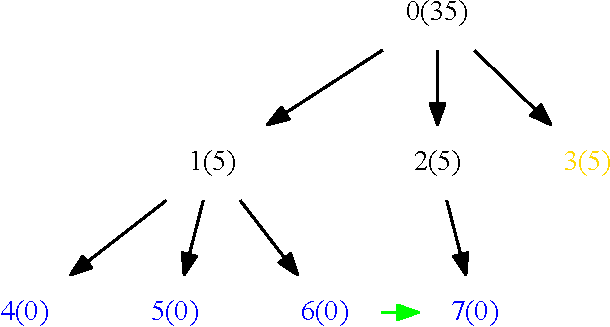
\includegraphics[width=.32\textwidth]{../paper/fig/0S1L.pdf}
\caption{0S-1L 求解分支图 (1秒)}
\end{figure}
\end{frame}

\dongtu{
\begin{frame}
\begin{figure}
\animategraphics[loop,autoplay,width=0.6\textwidth,poster=11]{8}{fig/(3+1)YTSF-100/}{001}{024}
\caption{(3+1)YTSF 方程的 0S-1L 解}
\end{figure}
\end{frame}
}

\begin{frame}{继承求解}
\begin{equation}
\begin{aligned}
    f_0 &= \sbrace{\xi_1+\eta_1}^2+\sbrace{\xi_2+\eta_2}^2+q_1\\ 
    f_1 &= \sbrace{\xi_1+\eta_1}^2+\sbrace{\xi_2+\eta_2}^2+q_1+q_2 \exp(\xi_3) 
\end{aligned}
\end{equation}
刚刚我们已经求得了$f_0$中系数之间的关系, 而$f_1$是包含$f_0$的, 所以可以将$f_0$的解代入$f_1$对应的方程组中, 以此类推, 从而简化高阶解的求解. 这就是继承求解. 
\end{frame}

\begin{frame}
\begin{figure}
\centering
\setcounter{subfigure}{0}
\subfigure[1S-1L直接求解(8秒)]{
    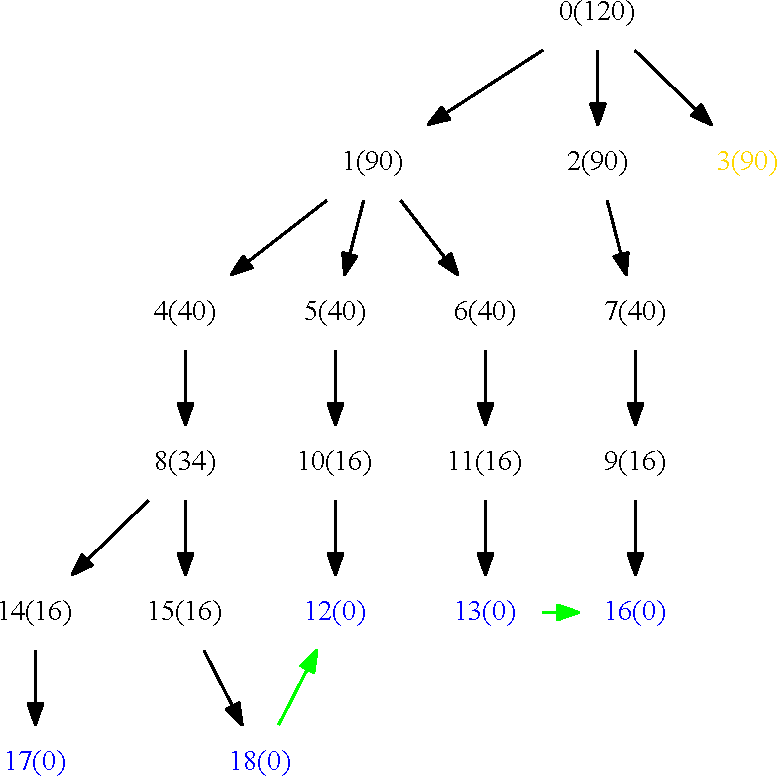
\includegraphics[width=.4\textwidth]{../paper/fig/1S1L-dir.pdf}
}
\hspace{2cm}
\subfigure[1S-1L继承求解(5秒)]{
    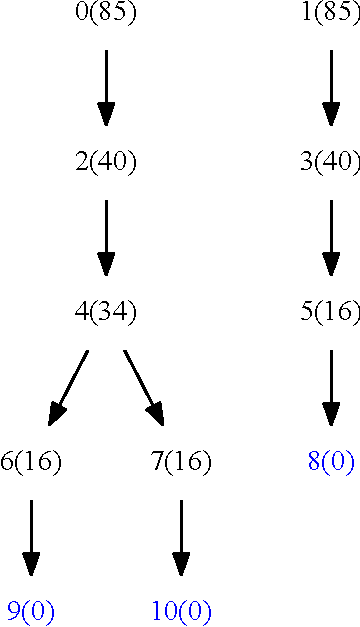
\includegraphics[width=.28\textwidth]{../paper/fig/1S1L-ext.pdf}
}
\end{figure}
\end{frame}

\dongtu{
\begin{frame}
\begin{figure}
\animategraphics[loop,autoplay,width=0.6\textwidth,poster=13]{8}{fig/(3+1)YTSF-101/}{001}{024}
\caption{(3+1)YTSF 方程的 1S-1L 解}
\end{figure}
\end{frame}
}

\begin{frame}
\begin{figure}
\centering
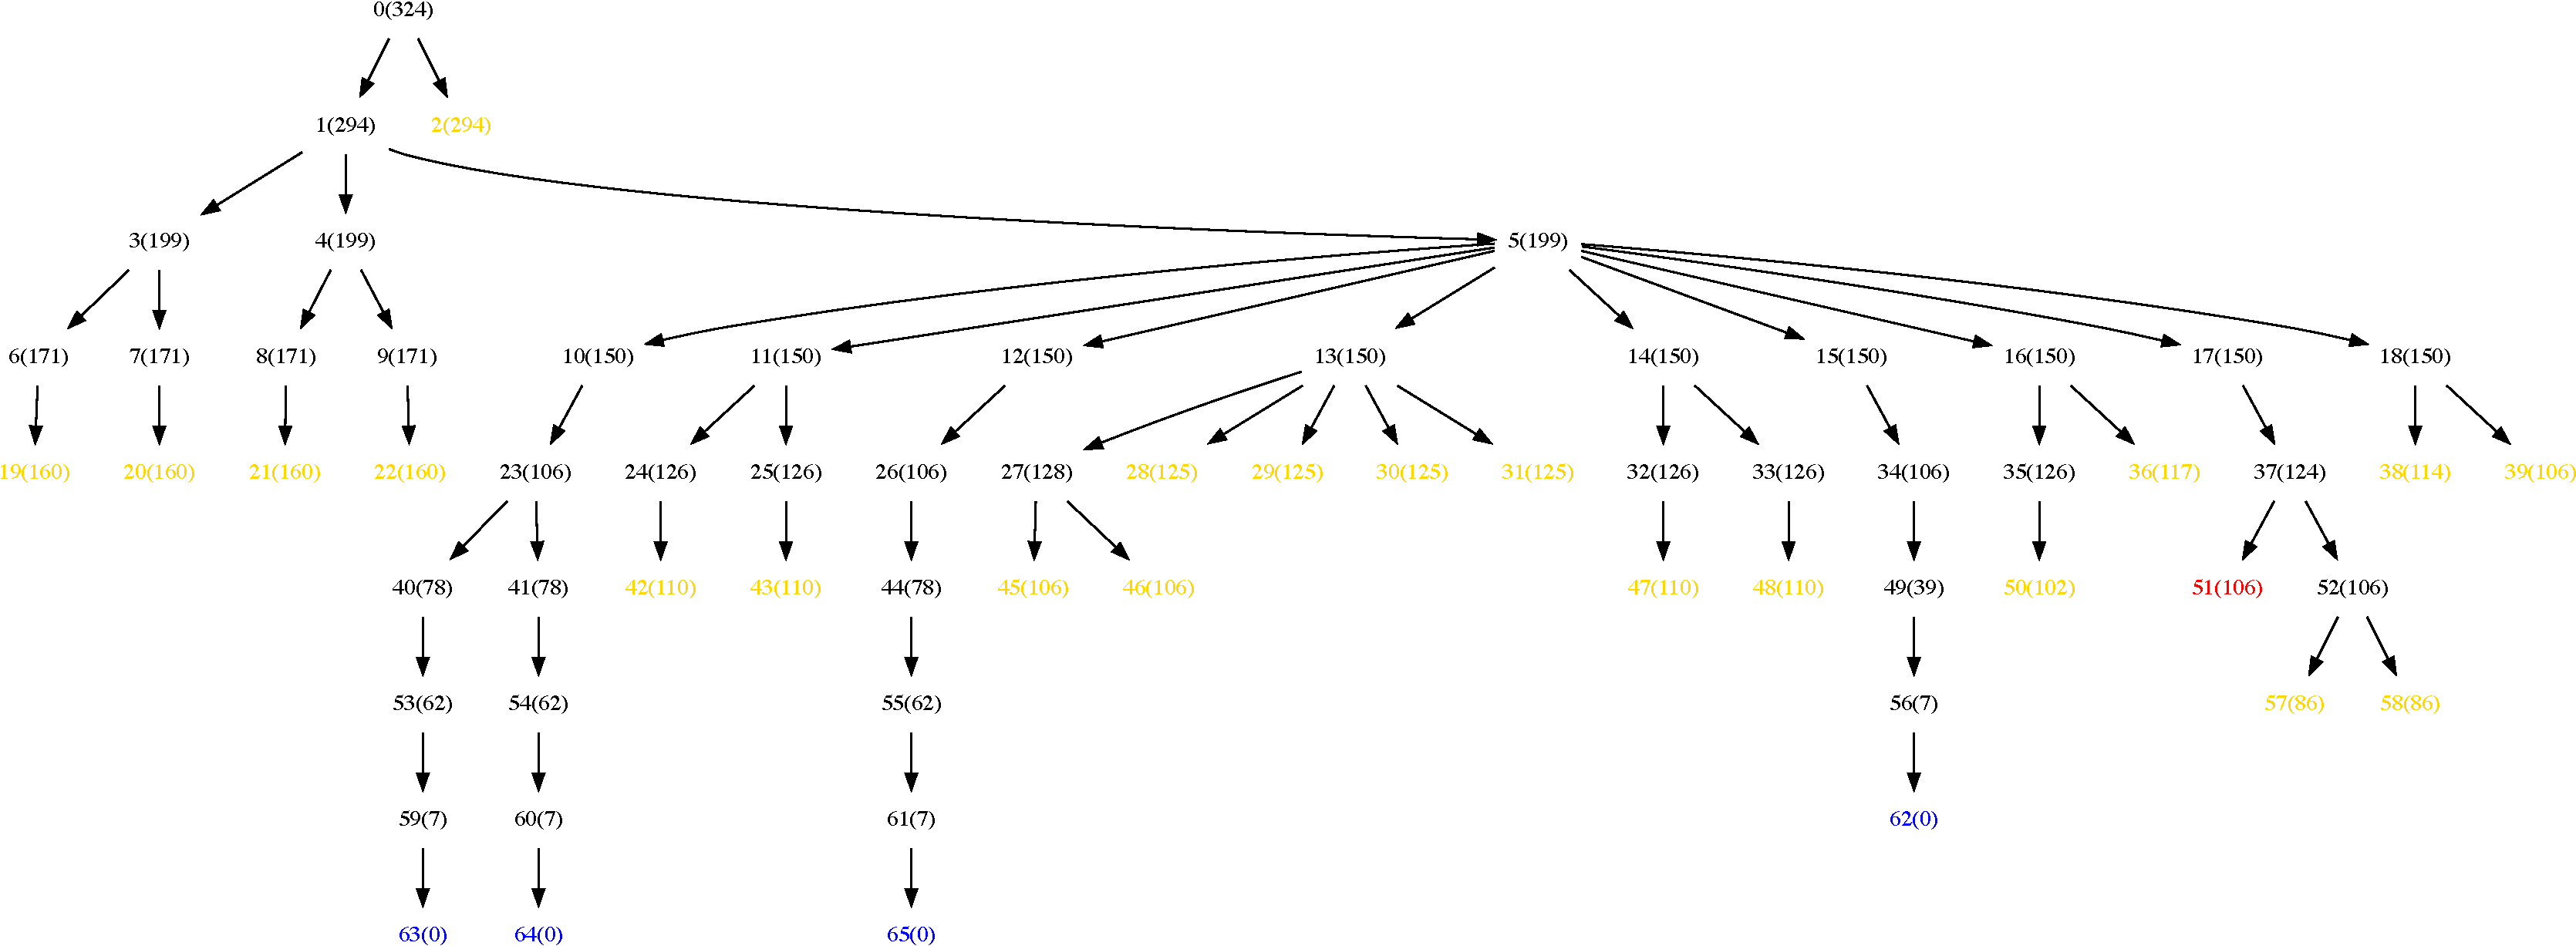
\includegraphics[width=\textwidth]{../paper/fig/2S1L-dir-TB-number.pdf}
\caption{2S-1L 直接求解的分支图(430 秒)}\label{sb2-d-n}
\end{figure}
\end{frame}

\frame{
\begin{figure}
\centering
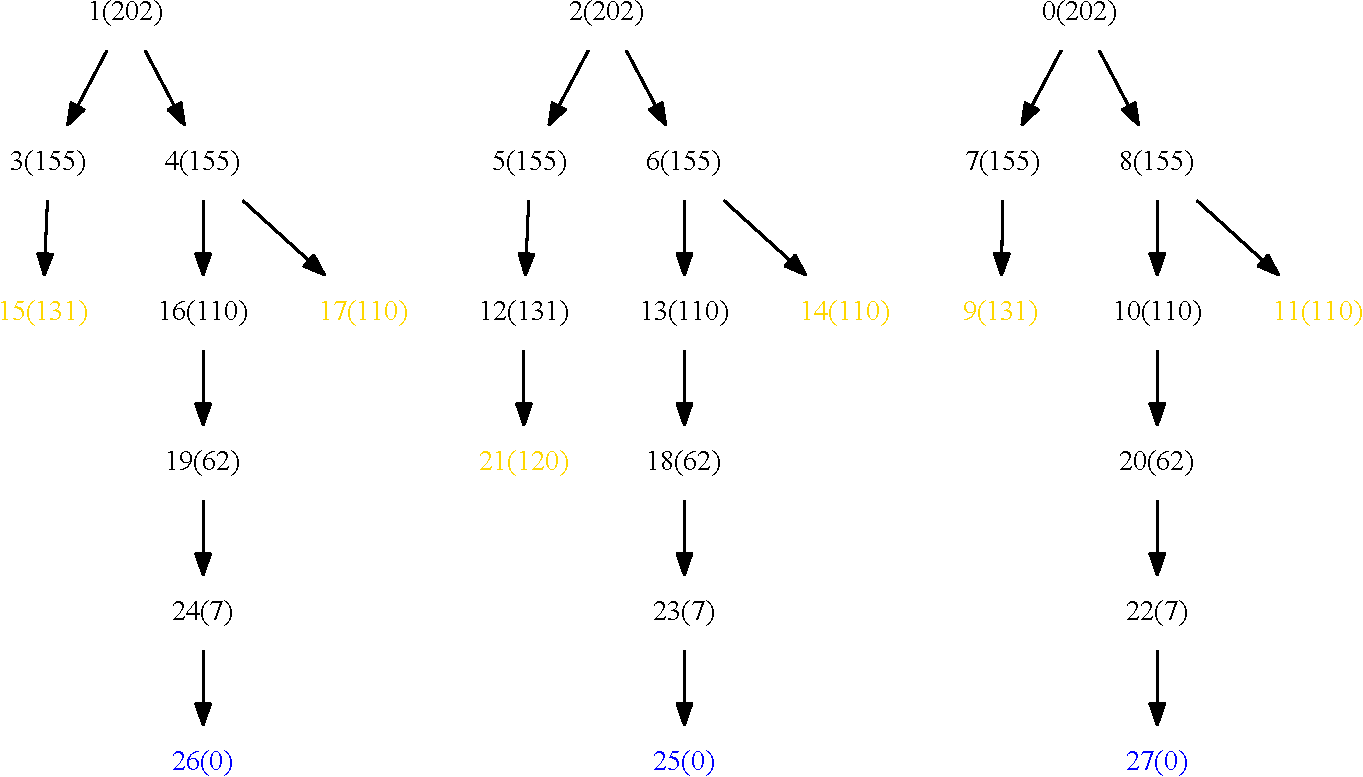
\includegraphics[width=\textwidth]{../paper/fig/2S1L-ext.pdf}
\caption{2S-1L 继承求解的分支图(30 秒)}\label{sb2-e}
\end{figure}
}

\dongtu{
\begin{frame}
\begin{figure}
\animategraphics[loop,autoplay,width=0.6\textwidth,poster=16]{8}{fig/(3+1)YTSF-102/}{001}{024}
\caption{(3+1)YTSF 方程的 2S-1L 解}
\end{figure}
\end{frame}
}

\subsection{求解效率对比}
\begin{frame}
\frametitle{求解效率对比}
\begin{adjustbox}{max width=\textwidth}
\centering
\renewcommand{\arraystretch}{1.3}
\begin{tabular}{cccccc}
\hline
来源方程 & 阶数 & 方程数 & 变量数 & PGSolve用时 & Solve用时 \\
\hline
(2+1) SK & 0 & 20 & 9 & 0.724 & 3.483 \\
(2+1) BKP-T & 0 & 20 & 9 & 0.571 & 3.486 \\
(2+1) KP & 0 & 35 & 9 & 1.759 & 29.643 \\
(3+1) YTSF & 0 & 35 & 11 & 1.229 & 8.839 \\
(3+1) JM & 0 & 35 & 11 & 0.845 & >1800 \\
(2+1) SK & 1 & 65 & 13 & 10.241 & >1800 \\
(3+1) YTSF & 1 & 120 & 16 & 12.228 & 1696.852 \\
\hline
\end{tabular}
\end{adjustbox}

\vspace{1em}

此处对比的是\cd{PDEtools:-Solve}. 而最常用的\cd{solve}函数甚至不能在 72 小时内求解只有 20 个方程的方程组, 这显然是\cd{solve}函数的一个 BUG.

\end{frame}

\begin{frame}

\begin{adjustbox}{max width=\textwidth}
\renewcommand{\arraystretch}{1.3}
\begin{tabular}{cccccc}
\hline
方程名称    & 解的阶数 & 方程数量 & 分组大小 & 解的个数 & 运行时间(s) \\ 
\hline 
(2+1)SK & 0 & 20 & 5 & 1 & 2.197 \\
(2+1)SK & 1 & 65 & 3 & 1 & 3.072 \\
(2+1)SK & 2 & 179 & 5 & 2 & 12.697 \\
(2+1)BKP-T & 0 & 20 & 5 & 1 & 1.036 \\
(2+1)BKP-T & 1 & 65 & 3 & 1 & 3.251 \\
(2+1)BKP-T & 2 & 179 & 5 & 2 & 12.617 \\
(3+1)YTSF & 0 & 35 & 5 & 2 & 1.948 \\
(3+1)YTSF & 1 & 120 & 5 & 3 & 6.717 \\
(3+1)YTSF & 2 & 324 & 5 & 3 & 37.909 \\
(3+1)JM & 0 & 35 & 5 & 3 & 2.014 \\
(3+1)JM & 1 & 120 & 5 & 13 & 18.384 \\
(3+1)JM & 2 & 324 & 5 & 4 & 50.934 \\
\hline 
\end{tabular}
\end{adjustbox}

\end{frame}

\section{n阶展开方法及其应用}
\begin{frame}{n阶展开方法及其应用}
\begin{columns}
\begin{column}{0.5\textwidth}
  \begin{figure}
    \centering
    \includegraphics[height=0.7\textheight]{fig/outline-p3.pdf}
  \end{figure}
\end{column}
\begin{column}{0.5\textwidth}
  \begin{enumerate}
  \item 齐次平衡原则
  \item 新的平衡点分类
  \item n阶展开方法
  \item 差分方程求解
  \item 双曲正切方法 
  \item \Painleve{}展开
  \end{enumerate}
\end{column}
\end{columns}
\end{frame}

\subsection{齐次平衡原则}
\begin{frame}{齐次平衡原则}
\[
    -x^4f(x+3)+(x+1)f(x)^2+8x^6+27x^5+28x^4+2x^3-x-1=0
\]
\[
    [m+4,2m+1,6]
\]
\[
    m\in \{2,3\} \Rightarrow \overline{m}=3
\]
\end{frame}

\subsection{新的平衡点分类}
\begin{frame}{新的平衡点分类}
\begin{figure}
\centering
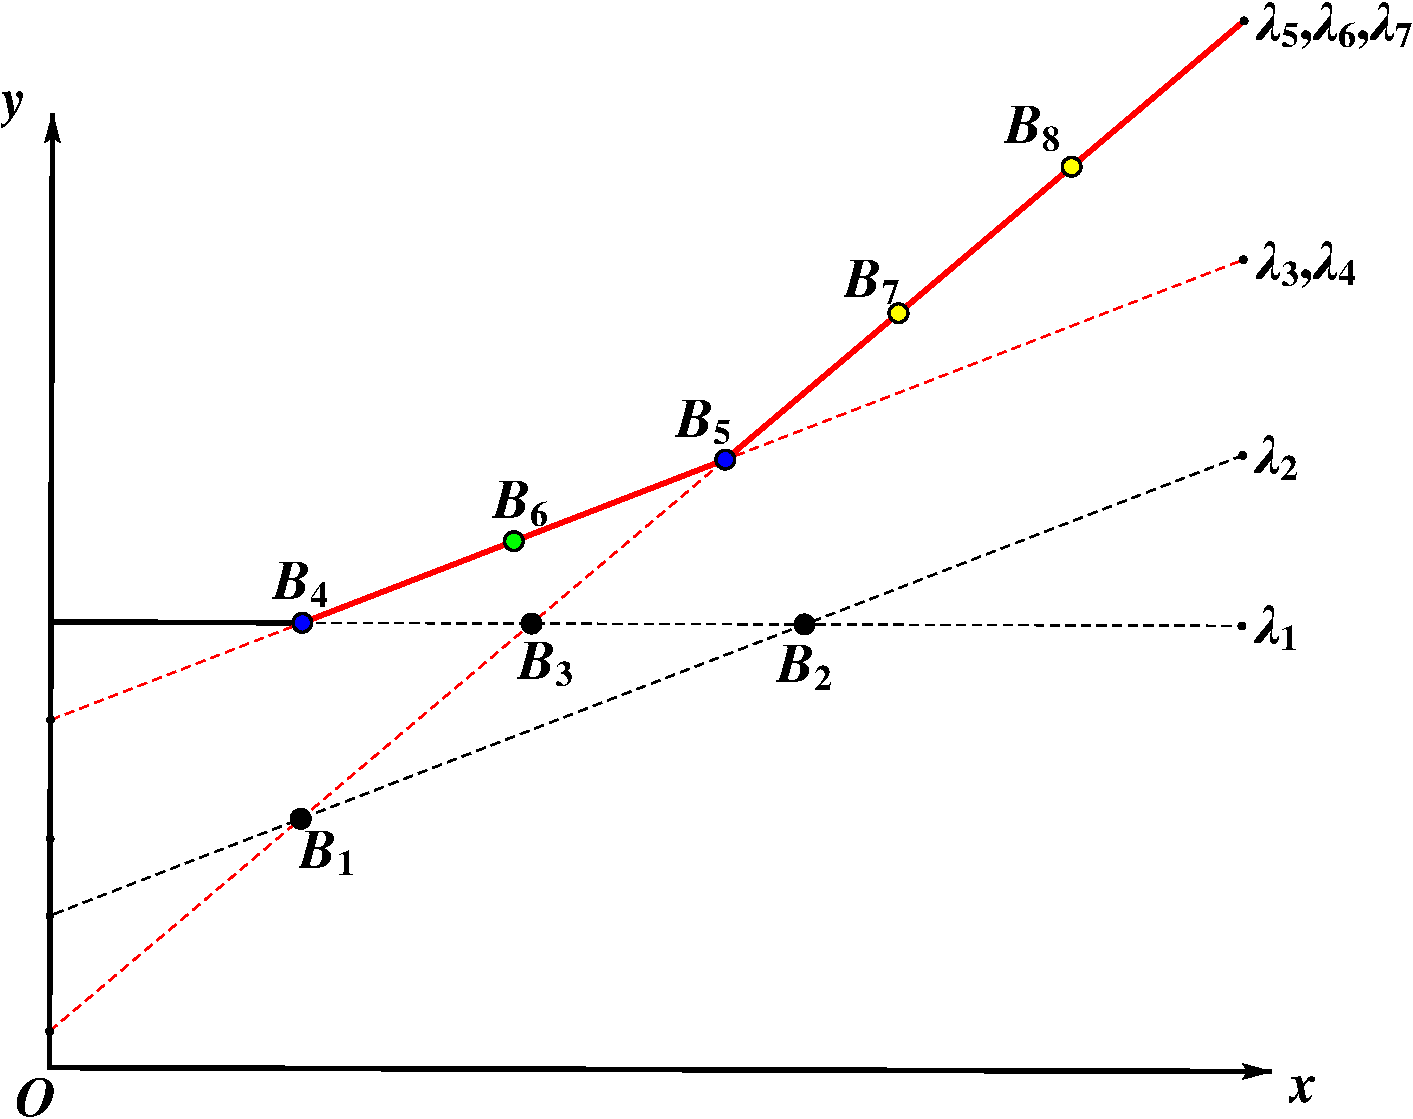
\includegraphics[height=0.8\textheight]{../paper/fig/ps.pdf}
\end{figure}
\end{frame}

\subsection{第二类平衡点}
\begin{frame}{第二类平衡点}
\small 
\[
    x^2f(x)f(x+1)f(x+2)+(1-x^9)f(x)+(x^4-x^9)f(x+1)+2x^9f(x+2)-\sum_{k=0}^{10}{c_k x^k}=0
\]
\[
    [c_0,\cdots,c_{10}]=[1,1,22,57,85,72,35,9,1,10,6]
\]
\[
    [3m+2,m+9,m+9,m+9,10]
\]
\[
    m+9=10 \Rightarrow m=1
\]
\[
    m+9 \ge \max\bbrace{3m+2,10} \Rightarrow m\le 7/2
\]
\[
    \overline{m}=3 \Rightarrow f(x)=x^2+x+1
\]
\end{frame}

\subsection{n阶展开方法}
\begin{frame}{n阶展开方法}
第三类平衡点, 平衡点有解 
\[
    (x+2)f(x)-(x-1)f(x+1)=0
\]
\[
    [m+1,m+1]
\]
\pause 
\[
    f(x)=u_0 x^m + u_1 x^{m-1} + \OO(x^{m-2})
\]
\[
    \OO\sbrace{x^n}=\left\{
    \begin{array}{cl}
    \text{次数不超过}\,n\,\text{的多项式} & n\ge 0, \\
    0                                    & n<0 .
    \end{array}
    \right.
\]
\[
    (-u_0 m+3u_0)x^m+\OO(x^{m-1})=0
\]
\[
    \overline{m}=3 \Rightarrow f(x)=c(x^3-x)
\]
\end{frame}

\begin{frame}
第三类平衡点, 平衡点无解
\[
    -2x^5f(x)f(x+2)+x^4f(x)^2+(2x^5-x^4)f(x+1)^2-\sum_{k=0}^{22}{c_k x^k}=0
\]
$[c_0,\cdots,c_{22}]$=[0, 0, 0, 0, 1, 2046, 10140, 22340, 28095, 20730, 7788, 6120, 30600, 84180, 151164, 199504, 199710, 151380, 85560, 35136, 10035, 1830, 170]
\[
    [2m+5,2m+4,2m+5,22]
\]
\[
    f(x)=u_0 x^m +\cdots +u_3 x^{m-3}+\OO(x^{m-4})
\]
\[
    \sbrace{ 2m^2u_0^2-3mu_0^2-2u_0u_1 } x^{2m+5-3}+\OO(x^{2m+5-4})=0
\]
只有当$2m+5-3>22$时, 上述加法才成立, 所以要使原方程有解, 需有
\[
    2m+5-3 \le 22 \Rightarrow m\le 10 \Rightarrow f(x)=\pm (x^{10}-1)
\]
\end{frame}

\subsection{双曲正切方法}
\begin{frame}{双曲正切方法}
\begin{equation*}
{{u}_{t}}+{{u}_{x}}+\alpha\,{{u}_{xxx}}+\beta\,u\,{{u}_{x}}+\gamma\,u\,{{u}_{xxx}}+\delta\,{{u}_{x}}\,{{u}_{xx}}=0. 
\end{equation*}
\[
  \xi=kx+ct+\eta
\]
\[
(c+k)u^\prime + \alpha k^3 u^{\prime\prime\prime}+\beta k u u^\prime+\gamma k^3 u u^{\prime\prime\prime}+\delta k^3 u^\prime u^{\prime\prime} = 0. 
\]
\pause 
\[
  T=\tanh(\xi), T^\prime=1-T^2 . 
\]
\[
  u=\sum_{k=0}^{m}{a_k T^{m-k}}
\]
\pause 
\[
  [m+1,m+3,2m+1,2m+3,2m+3]
\]
\[
  m+3=2m+3\Rightarrow m=0
\]
\end{frame}

\begin{frame}
\[
  u=a_m T^m + a_{m-1} T^{m-1} + \OO(T^{m-2})
\]
\[
  -{{{a}_{m}}}^{2}\,{k}^{3}\,m\,\left( m+1\right) \,\left( m\,\delta+\gamma\,m+2\,\gamma\right)T^{2m+3}+\OO(T^{2m+2})=0
\]
\[
  m=\frac{-2 \gamma}{\gamma+\delta}
\]
当$n\ge 1$时, 若$\gamma=-n,\delta=n+1$, 则$m=2n$, 原方程有解
\begin{equation*}
u=a_{2n} \sbrace{1-\tanh^2\sbrace{\pm\sbrace{\frac{\sqrt{-\beta}}{2n}x-\frac{\sqrt{-\beta}(\alpha\beta+n)}{2n^2}t}+\eta}}^n+\frac{\alpha}{n} . 
\end{equation*}
\end{frame}

\begin{frame}
取$\bbrace{a_{2n}=1,\alpha=1,\beta=-1,\eta=0}$进行绘图, 当$n=1,2,3$时, 其图像如下
\begin{figure}[ht]
\centering
\subfigure[$n=1$]{
    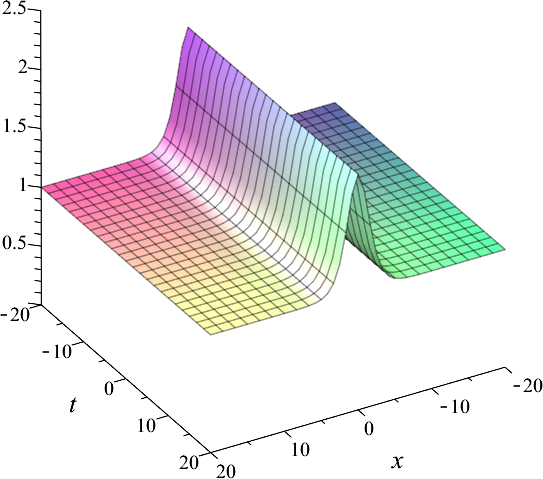
\includegraphics[width=.3\textwidth]{../paper/fig/(1+1)EMM-tanh-1.png}
}
\subfigure[$n=2$]{
    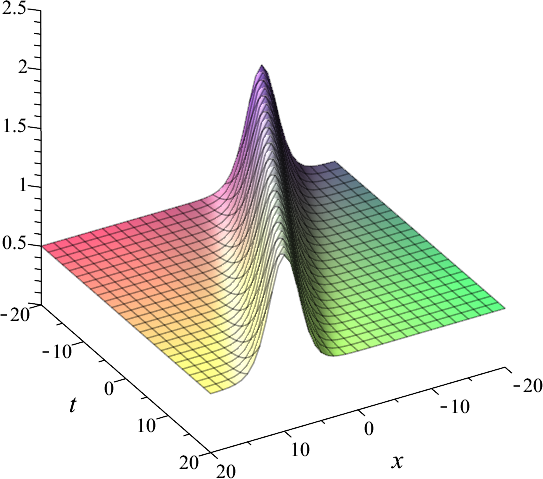
\includegraphics[width=.3\textwidth]{../paper/fig/(1+1)EMM-tanh-2.png}
}
\subfigure[$n=3$]{
    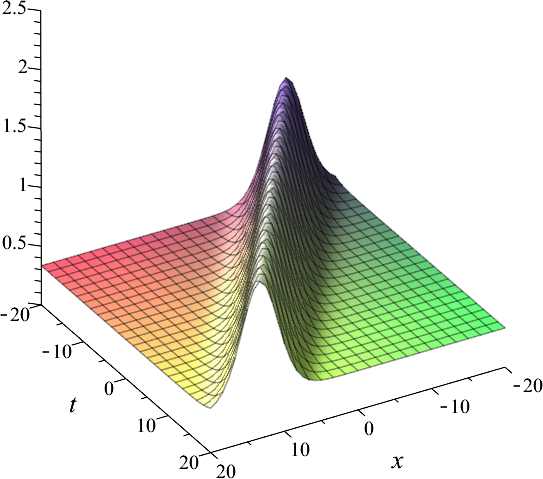
\includegraphics[width=.3\textwidth]{../paper/fig/(1+1)EMM-tanh-3.png}
}
\caption{(1+1)维EMM方程的双曲正切函数解} 
\end{figure}
\end{frame}

\subsection{\Painleve{}展开法}
\begin{frame}{\Painleve{}展开法}
\[
  u(u_t+u_{xxx})-3u_x u_{xx}=0.
\]
\[
  u=\sum_{k=1}^{m}\frac{u_k}{f^{m-k+1}}
\]
\[
  \DIF{x}{\frac{1}{f}}=-\frac{f_x}{f^2}
\]
\[
  \mbrace{2m+1,2m+3,2m+3}
\]
\[
  u=\frac{u_0}{f}+\OO(\frac{1}{f^2})
\]
\[
  2m(m^2-1)u_0^2f_x^3\frac{1}{f^{2m+3}}+\OO(\frac{1}{f^{2m+2}})=0
\]
\[
  m=1\Rightarrow u=\frac{F(t)\sqrt{f_x}}{f}
\]
\end{frame}

\section{积分化简}
\begin{frame}{积分化简}
\begin{columns}
\begin{column}{0.4\textwidth}
  \begin{figure}
    \centering
    \includegraphics[height=0.7\textheight]{fig/outline-p4.pdf}
  \end{figure}
\end{column}
\begin{column}{0.6\textwidth}
  \begin{enumerate}
  \item 非线性积分化简存在的问题
  \item 非线性积分多项式的线性化代数结构 
  \item 寻找化简规则 
  \item 转化为优化问题
  \item 典型例子 
  \end{enumerate}
\end{column}
\end{columns}
\end{frame}

\subsection{非线性积分化简存在的问题}
\begin{frame}{非线性积分化简存在的问题}
\[
    a=\int{u_x v \dd x},b=\int{u v_x \dd x},c=uv
\]
完全匹配
\[
    a+b=c
\]
非完全匹配
\[
    a+2b=c+b
\]
线性可约
\[
    a^2+2ab+b^2=c^2
\]
线性不可约
\[
    a^2+3ab+b^2=c^2+ab
\]
\end{frame}

\begin{frame}
嵌套积分
\[
    \int\!{\left(u\cdot\int\!{v_xw\dd x}+u\cdot\int\!{vw_x\dd x}\right)\dd x}=\int\!{uvw\dd x}
\]
积分视为导数
\[
    \int\!{\left(u\cdot\int\!{v\dd x}+\int\!{u\dd x}\cdot v\right)\dd x}=\int\!{u\dd x}\cdot\int\!{v\dd x}
\]
\end{frame}

\subsection{非线性积分多项式的线性化代数结构}
\begin{frame}{非线性积分多项式的线性化代数结构}
基本元素:
\[
\begin{aligned}
    f&=\underbrace{\int\!\int\!\cdots\!\int}_m{ \frac{\partial^n}{\partial v_1 \partial v_2 \cdots \partial v_n} (g_1 g_2 \cdots g_l)\dd u_1 \dd u_2 \cdots \dd u_m} \\ 
    &=\partial^U_V(G)
\end{aligned}
\]
化简对象:
\[
    I = \sum_{k=1}^N{c_k I_k}
\]
\end{frame}

\subsection{化简规则}
\begin{frame}{化简规则}
导数规则:
\[
    u_xvw+uv_xw+uvw_x=(uv)_xw+uvw_x=(uvw)_x
\]
乘法规则:
\[
    ab+ac+ad=a(b+c)+ad=a(b+c+d)
\]
都基于二项合并规则
\[
    I_1+I_2=I_3
\]
\end{frame}

\subsection{转化为优化问题}
\begin{frame}{转化为优化问题}
化简过程:
\[
\begin{aligned}
I &= \sum_{k=1}^N{c_k I_k}-\sum_{l=1}^L{x_l ({J_1}_l+{J_2}_l-{J_3}_l)} \\ 
& = \bm{B}(\bm{b}-\bm{A}\bm{x})
\end{aligned}
\]
优化问题:
\[
    \underset{\bm x}\min\VecNorm{\bm{b}-\bm{A}\bm{x}}_1
\]
线性规划模型:
\[
\begin{aligned}
    &\underset{\bm u,\bm x}\min \sum_{k=1}^L{u_k},\\
    &s.t. \left\{
    \begin{matrix}
    \bm{u}\ge \bm{b}-\bm{A}\bm{x},\\ 
    \bm{u}\ge \bm{A}\bm{x}-\bm{b},
    \end{matrix}
    \right.
\end{aligned}
\]
\end{frame}

\subsection{典型例子}
\begin{frame}{典型例子}
\[
\renewcommand{\arraystretch}{1.0}
\begin{array}{l}
-20u_xw_{xx}v
+c\ii{u_{xxxxx}\ii{v}}
+c\ii{u_{xxxxx}v}
+c\ii{v_{xxxxx}u}\\% 1
+20u_x^2v_xa
+20u_x\ii{wv_{xxx}}
+20w_x\ii{v_xu_{xx}}
+20w_x\ii{u_xv_{xx}}\\% 2
+10c\ii{v_{xxx}u^2}
+30c\ii{uu_xv_{xx}}
-20u_xwv_{xx}
-60cuu_x\ii{uv}\\% 3
+10c\ii{u_x\ii{u_xv_{xx}}}
+10c\ii{u_x\ii{v_xu_{xx}}}
-30vu^3c
-40u_xw_xv_x\\% 4
+30c\ii{u^2u_{xx}\ii{v}}
+20c\ii{v_xu_{xx}u}
+30c\ii{u_{xxx}u_x\ii{v}}\\% 5
+30c\ii{u_{xx}vu_x}
+40u_x\ii{w_xv_{xx}}
+40u_x\ii{v_xw_{xx}}
-120uu_xwv\\% 6
-4u_x^2v_xb
+20u_x\ii{vw_{xxx}}
+120u_x\ii{vuw_x}
+120u_x\ii{uvw_x}\\% 7
+60c\ii{uu_x^2\ii{v}}
+120c\ii{u^2u_xv}
-cuv_{xxxx}
-10u_{xxx}c\ii{vu}\\% 8
-10u_{xxx}c\ii{u_x\ii{v}}
-20u_xa\ii{u_xv_{xx}}
-20u_xa\ii{v_xu_{xx}}\\% 9
+4u_xb\ii{u_xv_{xx}}
-10cu\ii{u_xv_{xx}}
-10c v u u_{xx}
-10cu\ii{v_xu_{xx}}\\% 10
+4u_xb\ii{v_xu_xx}
+20c\ii{u_{xx}^2\ii{v}}
-cu_{xxxxx}\ii{v}\\% 11
+10c\ii{u_{xxxx}u\ii{v}}
+30u^2u_xc\ii{v}
-60uu_xc\ii{u_x\ii{v}}\\% 12
-20cu_xu_{xx}\ii{v}
+120u_x\ii{vwu_x}
+c\ii{u_xv_{xxxx}}
-10v_{xx}u^2c\\% 13
+30c\ii{u^3v_x}
+20c\ii{vu_{xxx}u}=0\\% 14
\end{array}
\]
\end{frame}

\begin{frame}{找到所有合并规则再化简的理由}
\[
\begin{array}{l}
0=\red{u_x\int\!{v_{xx}w_x\dd x}}+\red{u_x\int\!{v_xw_{xx}\dd x}}-\red{u_xv_xw_x}\\
~~+w_x\int\!{u_xv_{xx}\dd x}+w_x\int\!{u_{xx}v_x\dd x}-\red{u_xv_xw_x}\\
~~+u_x\int\!{vw_{xxx}\dd x}+\red{u_x\int\!{v_xw_{xx}\dd x}}-u_xvw_{xx}\\
~~+u_x\int\!{v_{xxx}w\dd x}+\red{u_x\int\!{v_{xx}w_x\dd x}}-u_xv_{xx}w ,
\end{array}
\]
如果事先合并了
\[
    u_x\int\!{v_xw_{xx}\dd x}+u_x\int\!{v_{xx}w_x\dd x}=u_xv_xw_x
\]
则无法继续合并剩余部分
\end{frame}

\begin{frame}{嵌套积分的多样性}
内部因式分解
\[
    c\int\!{\int\!{v\dd x}\,uu_{xxxx}\dd x}+c\int\!{\int\!{v\dd x}\,u_xu_{xxx}\dd x}=c\int\!{\int\!{v\dd x}\,(uu_{xxx})_x\dd x}
\]
积分视为导数
\[
    c\int\!{\int\!{v\dd x}\,(uu_{xxx})_x\dd x}+c\int\!{vuu_{xxx}\dd x}=cuu_{xxx}\int\!{v\dd x}
\]
\end{frame}

\section{总结}
\begin{frame}
\frametitle{总结}
\begin{figure}
\centering
\includegraphics[height=0.8\textheight]{fig/ppt-outline.pdf} 
\end{figure}
\end{frame}

\section{致谢}
\begin{frame}
\tikz[overlay,remember picture]\node[opacity=0.2]at (current page.center){
\includegraphics[width=0.7\paperheight]{../paper/sty/ecnu_logo.pdf}};
\centerline{\Huge 谢谢}
\end{frame}
\end{document}